%%
%% Author: jamie
%% 05/10/18
%%
\chapter{Implementation}\label{ch:development}
In this chapter the details of the product developed will be discussed.
This includes the implementation of the MCTS algorithm, our metric computation and
the development of our prototype game for demonstration purposes.


\section{UCT Algorithm}\label{sec:MCTS}
The core component of our implementation
\begin{lstlisting}[style=Python]

\end{lstlisting}

\subsection{Tree Representation}\label{subsec:treeRepresentation}

\subsection{Selection}\label{subsec:selection}

\begin{lstlisting}[style=Python]
def select(self, history):
    player = util.player(history)
    player_history = util.information_function(history, player)

    if player in {-1, 1}:
        tree = get_tree(player)
        eta_sub_expression = math.pow(1 + .1 * math.sqrt(tree[player_history].visitation_count), -1)
        eta = max((GAMMA, ETA_ZERO * eta_sub_expression))
        z = random.uniform(0, 1)
        if z < eta:
            return self.get_best_action_ucb(history, player, tree)
        else:
            return self.get_best_action_avg_strategy(player_history, tree)
    else:
        return random.choice(util.get_available_actions(history))
\end{lstlisting}


\begin{lstlisting}[style=Python]
def get_best_action_avg_strategy(self, player_history, tree):
    total_child_visits = 0
    actions = []
    probabilities = []

    for child in tree[player_history].children:
        total_child_visits += tree[child].visitation_count

    for child in tree[player_history].children:
        child_prob = tree[child].visitation_count / total_child_visits
        actions.append(child.replace(player_history, ""))
        probabilities.append(child_prob)

    return rand.choice(actions, p=probabilities)

\end{lstlisting}

\begin{lstlisting}[style=Python]
def get_best_action_ucb(self, history, player, tree):
    player_history = util.information_function(history, player)
    best_value = float('-inf')
    best_action = None

    for action in util.get_available_actions(history):
        node_val = self.calculate_next_node_value(tree, player_history, action, player)
        if node_val > best_value:
            best_action = action
            best_value = node_val

    return best_action
\end{lstlisting}


\subsection{Expansion}\label{subsec:expansion}

\begin{lstlisting}[style=Python]
def expand(tree, history, player):
    player_history = util.information_function(history, player)

    if player_history not in tree:
        tree[player_history] = potree.PoNode()

    for action in util.get_available_actions(player_history, player=player):
        new_history = player_history + action
        if new_history not in tree:
            tree[new_history] = potree.PoNode()
        tree[player_history].children.add(new_history)
\end{lstlisting}

\subsection{Simulation}\label{subsec:simulation}


\begin{lstlisting}[style=Python]
def simulate(self, history):
    if util.is_terminal(history):
        return self.handle_terminal_state(history)

    player = util.player(history)
    if self.out_of_tree[player]:
        return self.rollout(history)

    player_history = util.information_function(history, player)
    player_tree = get_tree(player)
    if player_history in player_tree and player_tree[player_history].children:
        action = self.select(history)
    else:
        expand(player_one_tree, history, 1)
        expand(player_two_tree, history, -1)
        action = random.choice(util.get_available_actions(history))
    if player != 0:
        self.out_of_tree[1] = True
        self.out_of_tree[-1] = True

    new_history = history + action
    running_reward = evaluator.calculate_reward_full_info(history) + \
                         self.discount_factor * self.simulate(new_history)
    update_player_tree(history, action, 1, running_reward)
    update_player_tree(history, action, -1, running_reward)

    return running_reward
\end{lstlisting}


\begin{lstlisting}[style=Python]
def rollout(self, history):
    action = random.choice(util.get_available_actions(history))
    new_history = history + action
    return self.simulate(new_history)
\end{lstlisting}

\subsection{Tree Update}\label{subsec:treeUpdate}

\begin{lstlisting}[style=Python]
def update(tree, history, new_history, running_reward):
    tree[history].visitation_count += 1
    tree[new_history].visitation_count += 1
    tree[new_history].value += (running_reward - tree[new_history].value) / tree[new_history].visitation_count
\end{lstlisting}

\section{Best Response Computation}\label{sec:bestResponseComputation}
In order to evaluate the performance of our agent exploitability was utilised as the primary metric.
Exploitability is a measure of how well our agent would fare against an opponent responding
optimally to our strategy.
Exploitability is related to the concept of Nash equilibria in that a Nash equilibrium
is induced by a strategy that cannot be exploited.

To calculate the exploitability of a strategy the best responses to that strategy must be
determined.
The first step in calculating the best response strategy involves
taking our agent's action selections and inserting them into the game tree\citep{heinrich2017reinforcement}.
In other words, wherever the agent must take an action in the game tree, the best action is chosen
based on our MCTS estimations.
As such the resultant tree will consist of the MCTS player's decision nodes which will have
a single child node along with the second player's decision nodes and chance nodes
which will both have multiple children.
Terminal states can then be evaluated followed by propagation of values back up the tree, with the highest
child value being propagated when a decision node for player two is reached.
The average child value is propagated for chance nodes.
This process will now be explained in detail with coding examples.

\subsection{Generating Best Response Tree}\label{subsec:applyMCTS}

\begin{figure}[ht]
    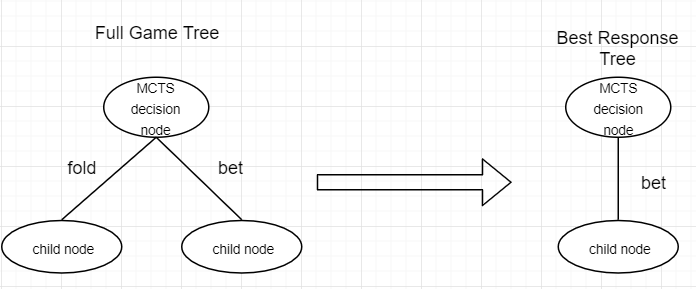
\includegraphics[scale=1]{images/best_response_tree_vs_full_tree.PNG}
    \caption{Generation of Best Response Tree}
\end{figure}

\subsection{Propagating Terminal Values}\label{subsec:propagateTerminals}
\subsection{Exploitability}\label{subsec:exploitability}

\section{Prototype Application}\label{sec:prototypeApp}
In order to give visual evidence of the work done and the agent developed, a user interface(UI) was created
that allowed human interaction with the trained bot.
In order to facilitate the development of this interface in a short period of time the Qt framework was used.
Qt is a open-source widget toolkit for creating graphical user interfaces and applications.
Specifically Qt Designer was used in order to generate a UI template.
Qt Designer is a what-you-see-is-what-you-get (WYSIWYG) UI generation tool that accompanies Qt.
PyQt5 was then used to generate python code from this UI template and connect the functional component of the game.
In this section the process involved in creating this prototype application will be outlined
and some key code snippets will be highlighted.

In order to elicit requirements for this application I applied brainstorming as well as analysing a number
of online UIs that served a similar purpose to mine.
This process rendered the following functional requirements:
\begin{itemize}
    \item Display list of available actions.
    \item Allow user to take action.
    \item Display relevant cards to player.
    \item Annotate the sequence of events that occur in the game.
    \item Display the current pot size.
    \item Allow player to play multiple rounds.
    \item Keep track of cumulative winnings across multiple rounds.
\end{itemize}

\subsection{UI Screen}\label{subsec:UiScreen}
The first step towards achieving these functional requirements was to generate a UI screen.
This was achieved through Qt designer using drag and drop with the end result being as shown below.
Due to the fact that a number of images had to be displayed for the available cards in the
game a Qt resource file was also created to store and locate those images.

\begin{figure}[ht]
    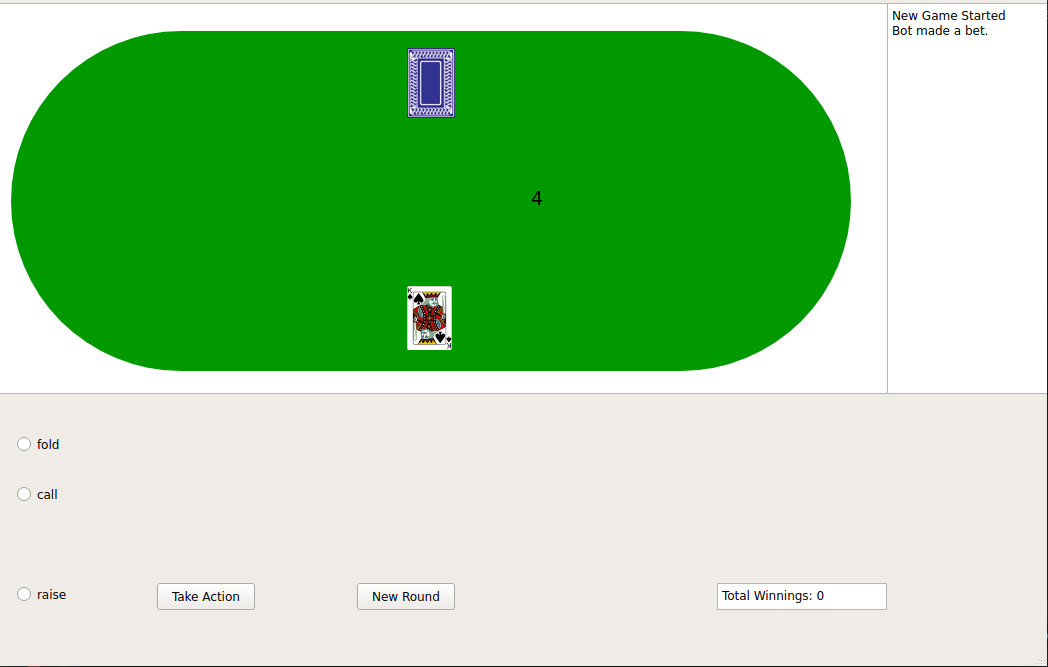
\includegraphics[scale=.4]{images/UI_screenshot.png}
    \caption{Game UI}
\end{figure}

Qt designer generates a .ui file that stores the UI template as well as a .qrc resource file.
The following commands were used to convert these two files into python format in order for them
to be compatible with the rest of the program:
\begin{lstlisting}[language=bash]
$ pyuic4 -x ui.ui -o screen.py
$ pyrcc4 -o cards_resource.py cards/cards_resource.qrc
\end{lstlisting}

In order to create a visible screen the following code was used:

\begin{lstlisting}[style=Python]
def setup_screen(self):
    self.main_window = QMainWindow()
    self.ui_screen = screen.Ui_MainWindow()
    self.ui_screen.setupUi(self.main_window)
    self.main_window.show()
    sys.exit(self.application.exec_())
\end{lstlisting}

\subsection{Event Handling and UI Manipulation}\label{subsec:eventHandling}
When the UI screen had been implemented it was then time to attach the screen to the
functional aspect of the game.
This was done through the creation of a python class called Controller that extends the QWidget
class from the PyQt framework.

In order to handle events callback methods were registered with the buttons that required their events to be handled.
The code below demonstrated this process:
\begin{lstlisting}[style=Python]
def setup_event_handlers(self):
    self.ui_screen.take_action_button.clicked.connect(self.take_action)
    self.ui_screen.new_game_button.clicked.connect(self.new_game)
\end{lstlisting}

Along with event handling the Controller class also had the responsibility of updating the
UI based on the information that it gained from the game model, which will be discussed in the next section.
This primarily involved calling the setText() method of a number of the screen's widgets.

\subsection{Game Model}\label{subsec:gameModel}
The third component of our game was the game model.
This was instantiated through a python class named Model that had the responsibility of feeding
the correct data to the Controller class at any point in the game.
Due to the fact there was already significant functionality built around the concept of histories,
it was decided that the state of the game would be tracked through the use of histories.
From the history the majority of the information about the game could be deciphered.
This included the available actions, the cards in play and the pot.
In order to fully satisfy our functional requirements the Model class also kept track of annotation messages
that were generated based on game events, along with the cumulative winnings of the player over time.
This data was returned to the Controller class in the
form of a python dictionary.

The most significant method in this class was the update\_game\_state method.
This method handled the player taking actions, the agent responding to those actions and the state being
updated.
Below the code for this method is listed.

\begin{lstlisting}[style=Python]
def update_game_state(self, action, player):
    self.history += action
    self.display_text += PLAYER_NAMES[player] + ACTION_MESSAGES[action]

    # Handle the game being over
    if util.is_terminal(self.history):
        winner = evaluator.get_winner(self.history)
        winnings = -evaluator.calculate_reward_full_info(self.history)
        self.total_winnings += winnings
        self.display_text += "Game over. " + PLAYER_NAMES[winner] + "won: " + str(abs(winnings))

    # If the next player is the bot, allow it to take its action
    elif util.player(self.history) == 1:
        self.update_game_state(self.agent.get_action(self.history), 1)

    # If the we need cards to be dealt, deal the cards.
    elif util.player(self.history) == 0:
        self.pub_card = random.choice(util.get_available_cards(self.history))
        self.update_game_state(self.pub_card, 0)
\end{lstlisting}

\subsection{Agent Representation}\label{subsec:agent}
In the case of this prototype game the agent is merely an instantiation of a pre-defined strategy.
As such when we call agent.get\_action(history) in the previous code block we are either stochastically
or deterministically selecting an action based the aforementioned strategy.

